\noindent The story so far
\begin{itemize}
\item Built a free (non-interacting) relativistic quantum field theory, namely, the Klein-Gordon field, with Hamiltonian $\hat{H}_{KG}$.

\item Added (Lorentz invaraint) interactions via the Hamiltonian
	\subitem \begin{equation} \hat{H}_{int} = \frac{\lambda}{4!} \int d^3 x \, \hat{\phi}^4(\textbf{x}), \, \lambda >> 1 \end{equation}.

\item Used perturbation theory to solve the Hamiltonian $\hat{H} = \hat{H}_{KG} + \hat{H}_{int}$.

\item Studied observable quantities via the $n$-point correlation function
	\subitem \begin{equation} G^{(n)}(\textbf{x}_1, \dots, \textbf{x}_n) = \bra{\Omega} \mathcal{T}[\hat{\phi}_H(\textbf{x}_1) \dots \hat{\phi}_H(\textbf{x}_n) ] \ket{\Omega} \end{equation}.
	\subitem Where $\ket{\Omega}$ is the full, interacting vacuum state, and $\hat{\phi}_H(\textbf{x}_i) = \hat{\phi}_{iH} = \hat{\phi}_I(\textbf{x}_i) = \hat{\phi}_{iI}$ is the field operator in the Heisenberg, interaction, picture, where the observables (e.g., field operators) closer to direct observation.

\item Claimed and "proved" that the $n$-point correlation function can be calculated in terms of the ground state expectation values of the field operators, and the scattering $\mathcal{S}$-matrix .
	\subitem \begin{equation} G^{(n)}(\textbf{x}_1, \dots, \textbf{x}_n) = \frac{\bra{0} \mathcal{T}[\hat{\phi}_{1I} \dots \hat{\phi}_{nI} \mathcal{S} ]\ket{0} }{\bra{0} \mathcal{S} \ket{0}} \end{equation}
	\subitem Where $\bra{\phi}\mathcal{S}\ket{\psi} = \lim_{t\to\infty} \bra{\phi} \mathcal{T}[e^{-i \int^t_{-t} \hat{H}_{int}(t') dt'}] \ket{\psi}, \, \forall \ket{\phi}, \ket{\psi}$
\end{itemize}

\noindent Now, to calculate quantities like the numerator of the $n$-point correlation function consider the field operator in the interaction picture (dropping the subscript "$I$")
\begin{equation}
\hat{\phi}_I(\textbf{x}) = \hat{\phi}(\textbf{x}) = \int \frac{d^3 p}{\sqrt{2 \omega_p}} (\hat{a}_\textbf{p} e^{-i \textbf{p} \cdot \textbf{x}} + \hat{a}^\dagger_\textbf{p} e^{i \textbf{p} \cdot \textbf{x}} ) = \hat{\phi}^+(\textbf{x}) + \hat{\phi}^-(\textbf{x})
\end{equation}

\noindent Where $\textbf{p} = (\omega_p, p)$, with $\omega_p = \sqrt{p^2 + m^2}$, such that $\textbf{p}\cdot\textbf{x} = p^0x^0 - p\cdot x$, and the newly defined operators annihilate the ground state, such that 
\begin{equation} 
\hat{\phi}^+(\textbf{x})\ket{0} = 0 \,\,\,\, \text{and} \,\,\,\, \bra{0}\hat{\phi}^-(\textbf{x}) = 0. 
\end{equation}

\noindent For example, consider the time-ordering of the two particle case (note the notation change for the four-vector in this section $\textbf{x} \rightarrow x$)
\begin{align*}
\mathcal{T}[\hat{\phi}(x)\hat{\phi}(y)]_{x^0>y^0} &= \hat{\phi}(x)\hat{\phi}(y) \\
&= \hat{\phi}^+(x)\hat{\phi}^+(y) + \hat{\phi}^+(x)\hat{\phi}^-(y) \\
&\,\,\,\,\,\, + \hat{\phi}^-(x)\hat{\phi}^+(y) + \hat{\phi}^-(x)\hat{\phi}^-(y) \\
&= \hat{\phi}^+(x)\hat{\phi}^+(y) + \left(\hat{\phi}^-(y)\hat{\phi}^+(x) + [\hat{\phi}^+(x), \hat{\phi}^-(y)]\right) \\
&\,\,\,\,\,\, + \hat{\phi}^-(x)\hat{\phi}^+(y) + \hat{\phi}^-(x)\hat{\phi}^-(y)  \\ 
\mathcal{T}[\hat{\phi}(x)\hat{\phi}(y)]_{x^0>y^0} &= \hat{\phi}^+(x)\hat{\phi}^+(y) + \left(\hat{\phi}^-(y)\hat{\phi}^+(x) + D(x-y)\cdot\mathbb{I}\right) \\
&\,\,\,\,\,\, + \hat{\phi}^-(x)\hat{\phi}^+(y) + \hat{\phi}^-(x)\hat{\phi}^-(y) 
\end{align*}

\noindent Then the ground state expectation value of two interacting field operators is simply the Feynman propagator
\begin{align}
\bra{0} \mathcal{T}[\hat{\phi}(x)\hat{\phi}(y)] \ket{0} &= \Delta_F(x-y) \\
&= i \int \frac{d^4 p}{(2\pi)^4} \frac{e^{-i p\cdot(x-y)}}{p^2 - m^2 + i\epsilon} \,\, , \,\, \epsilon>0 \\
&=
	\begin{cases}
      		D(x-y), & x^0 > y^0 \\
      		D(y-x), & x^0 \le y^0
    	\end{cases}
\end{align}

\subsection*{Wick Contraction and Normal Ordering}

\noindent Introduce some notation for extracting Feynman propagators from quantities like the expectation value of time-ordered field operators, called the \textbf{Wick contraction}. For two field operators, $\hat{\phi}(x)$ and $\hat{\phi}(y)$, and any three other operators $\hat{A}$, $\hat{B}$, and $\hat{C}$, write 
\begin{align}
\wick[offset=1.5em]{\c {\hat{\phi}(x)} \c {\hat{\phi}(y)}} &= \Delta_F(x-y) \cdot \mathbb{I} \\
\wick[offset=1.5em]{A \c {\hat{\phi}(x)} B \c {\hat{\phi}(y)} C} &= \Delta_F(x-y) \cdot \hat{A}\hat{B}\hat{C}
\end{align}

\noindent Also introduce \textbf{normal ordering}, denoted by $\mathcal{N}[\,]$ that sends all "dagger" operators to the left. For example,
\begin{equation}
\mathcal{N}[\hat{a}_p \hat{a}_q^\dagger \hat{a}_r \hat{a}_s^\dagger ] = \hat{a}_q^\dagger \hat{a}_s^\dagger \hat{a}_p \hat{a}_r
\end{equation}

\noindent Observe the relationship between time-ordering and normal-ordering using the Wick contraction
\begin{align}
\mathcal{T}[\hat{\phi}(x) \hat{\phi}(y)] &= \mathcal{N}[\hat{\phi}(x) \hat{\phi}(y) + \Delta_F(x-y)\cdot\mathbb{I}] \\
&= \mathcal{N}[\hat{\phi}(x) \hat{\phi}(y) + \wick[offset=1.5em]{\c {\hat{\phi}(x)} \c {\hat{\phi}(y)}}
\end{align}

\noindent A more involved example of the time-ordering of four field operators, where the only nonzero terms at the end of acting on states will be the "double contractions", since 
\begin{align*}
\mathcal{T}[\hat{\phi}(x_1) \hat{\phi}(x_2) \hat{\phi}(x_3) \hat{\phi}(x_4)] &= \mathcal{N}[\hat{\phi}_1 \hat{\phi}_2 \hat{\phi}_3 \hat{\phi}_4 + \text{"all possible contractions"}]\\
&= \mathcal{N}[\hat{\phi}_1 \hat{\phi}_2 \hat{\phi}_3 \hat{\phi}_4 + \wick[offset=1.5em]{\c {\hat{\phi}_1} \c {\hat{\phi}_2} \hat{\phi}_3 \hat{\phi}_4} + \wick[offset=1.5em]{\c {\hat{\phi}_1} {\hat{\phi}_2} \c {\hat{\phi}_3} \hat{\phi}_4} \\
&\,\,\,\,\,\, + \wick[offset=1.5em]{\c {\hat{\phi}_1} {\hat{\phi}_2} {\hat{\phi}_3} \c {\hat{\phi}_4}} + + \wick[offset=1.5em]{{\hat{\phi}_1} \c {\hat{\phi}_2} \c {\hat{\phi}_3} {\hat{\phi}_4}} + \wick[offset=1.5em]{{\hat{\phi}_1} {\hat{\phi}_2} \c {\hat{\phi}_3} \c {\hat{\phi}_4}} + \wick[offset=1.5em]{{\hat{\phi}_1} \c {\hat{\phi}_2} {\hat{\phi}_3} \c {\hat{\phi}_4}} \\
&\,\,\,\,\,\, + \wick[offset=1.5em]{\c1 {\hat{\phi}_1} \c2 {\hat{\phi}_2} \c1 {\hat{\phi}_3} \c2 {\hat{\phi}_4}} + \wick[offset=1.5em]{\c1 {\hat{\phi}_1} \c2 {\hat{\phi}_2} \c2 {\hat{\phi}_3} \c1 {\hat{\phi}_4}} + \wick[offset=1.5em]{\c1 {\hat{\phi}_1} \c1 {\hat{\phi}_2} \c2 {\hat{\phi}_3} \c2 {\hat{\phi}_4}} ]
\end{align*}

\noindent The ground state matrix elements of $\mathcal{T}[\hat{\phi}_1 \hat{\phi}_2 \hat{\phi}_3 \hat{\phi}_4]$ is then
\begin{align*}
\bra{0} \mathcal{T}[\hat{\phi}_1 \hat{\phi}_2 \hat{\phi}_3 \hat{\phi}_4] \ket{0} &= \cancel{\bra{0} \mathcal{N}[\hat{\phi}_1 \hat{\phi}_2 \hat{\phi}_3 \hat{\phi}_4] \ket{0}} + \cancel{\bra{0} \mathcal{N}[\wick[offset=1.5em]{\c {\hat{\phi}_1} \c {\hat{\phi}_2} \hat{\phi}_3 \hat{\phi}_4}] \ket{0}} + \cancel{\dots} \\
&\,\,\,\,\,\, + \Delta_F(x_1-x_2)\Delta_F(x_3-x_4) + \Delta_F(x_1-x_3)\Delta_F(x_2-x_4) \\
&\,\,\,\,\,\, + \Delta_F(x_1-x_4)\Delta_F(x_2-x_3)
\end{align*}

\noindent Where these are the values of the associated Feynman diagrams, which we write down in a "reverse" way, extracting the diagram from the calculated value. Later, we will extract the values from the diagrams.

\begin{figure}[H]
	\centering
	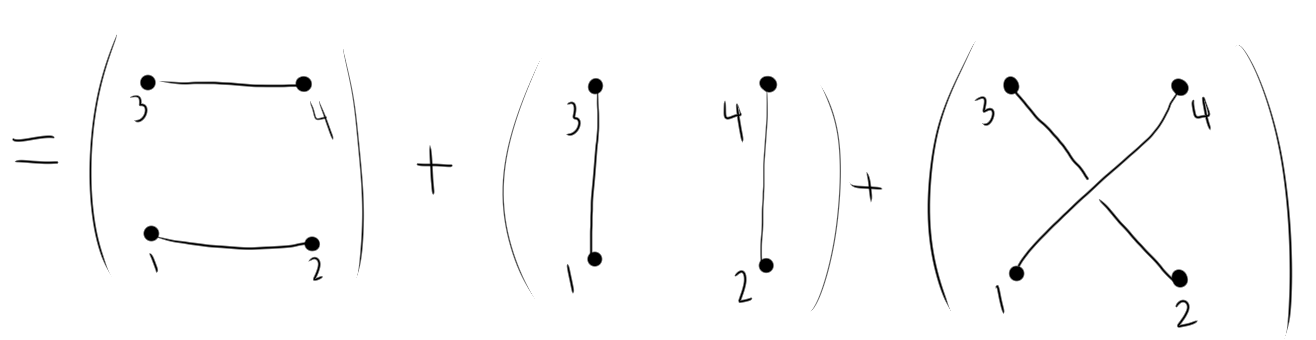
\includegraphics[scale=0.5]{feynman1.png}
	\caption{Feynamn diagrams representing the nonzero values in the four particle example above.}
\end{figure}

\noindent Now stated in its general form \\

\noindent \textbf{Wick's Theorem}: $\mathcal{T}[\hat{\phi}_1 \dots \hat{\phi}_n] = \mathcal{N}[\hat{\phi}_1 \dots \hat{\phi}_n + \text{"all possible contractions"}]$. \\

\noindent \textbf{Proof:} \\
\noindent Induct on $n$, with the base case $n=2$ confirmed to be true, and check that the $n-1$ case implies the full $n$ case. \\
\noindent Assume, without loss of generality, that everything is time-ordered, such that $x_1^0 > x_2^0 > \dots > x_n^0$. \\
\noindent Then the left-hand side of Wick's theorem becomes
\begin{equation}
\mathcal{T}[\hat{\phi}_1 \dots \hat{\phi}_n] = \hat{\phi}_1 \hat{\phi}_2 \dots \hat{\phi}_n .
\end{equation}
\noindent Use the inductive hypothesis for $n-1$ case on this equation
\begin{align*}
\hat{\phi}_1 \hat{\phi}_2 \dots \hat{\phi}_n &= (\hat{\phi}_1^+ + \hat{\phi}_1^-) \mathcal{N} [ \hat{\phi}_2 \dots \hat{\phi}_n + \left(\text{\stackanchor{{\small all possible contractions}}{{\small excluding $\hat{\phi}_1$.}}}\right) ] \\
&= \hat{\phi}_1^+ \mathcal{N}[\hat{\phi}_2 \dots \hat{\phi}_n + \left(\text{\stackanchor{{\small all possible contractions}}{{\small excluding $\hat{\phi}_1$.}}}\right)] \\
&\,\,\,\,\,\, + \mathcal{N}[ \hat{\phi}_1^- \hat{\phi}_2 \dots \hat{\phi}_n + \hat{\phi}_1^- \left(\text{\stackanchor{{\small all possible contractions}}{{\small excluding $\hat{\phi}_1$.}}}\right) ] .
\end{align*}
\noindent Since $\hat{\phi}_1^-$ is already normal-ordered. \\
\noindent Focus on the first part of the first term of $\hat{\phi}_1 \hat{\phi}_2 \dots \hat{\phi}_n$ above
\begin{align*}
\hat{\phi}_1^+ \mathcal{N}[\hat{\phi}_2 \dots \hat{\phi}_n] &= \mathcal{N}[\hat{\phi}_2 \dots \hat{\phi}_n] \hat{\phi}_1^+ + [\hat{\phi}_1^+, \mathcal{N}[\hat{\phi}_2 \dots \hat{\phi}_n]] \\
&= \mathcal{N}[\hat{\phi}_1^+ \hat{\phi}_2 \dots \hat{\phi}_n] \\
&\,\,\,\, + \mathcal{N}[ [\hat{\phi}_1^+, \hat{\phi}_2]\hat{\phi}_3 \dots \hat{\phi}_n + \hat{\phi}_2 [\hat{\phi}_1^+,\hat{\phi}_3] \hat{\phi}_4 \dots \hat{\phi}_n + \dots + \hat{\phi}_2\hat{\phi}_3\dots\hat{\phi}_{n-1}[\hat{\phi}_1^+,\hat{\phi}_n]] \\
\hat{\phi}_1^+ \mathcal{N}[\hat{\phi}_2 \dots \hat{\phi}_n] &= \mathcal{N}[ \hat{\phi}_1^+ \hat{\phi}_2 \dots \hat{\phi}_n + \wick[offset=1.5em]{\c {\hat{\phi}_1^+} \c {\hat{\phi}_2} \hat{\phi}_3 \dots \hat{\phi}_n} + \wick[offset=1.5em]{\c {\hat{\phi}_1^+} {\hat{\phi}_2} \c {\hat{\phi}_3} \dots \hat{\phi}_n} + \dots + \wick[offset=1.5em]{\c {\hat{\phi}_1^+} {\hat{\phi}_2} \hat{\phi}_3 \dots \c {\hat{\phi}_n}} ] .
\end{align*}
\noindent Where the second equality follows from $[\hat{\phi}_j^\dagger, \hat{\phi}_k] \propto \mathbb{I}$. \\
\noindent Now, focus on the rest of the first term of $\hat{\phi}_1 \mathcal{N}[\hat{\phi}_2 \dots \hat{\phi}_n]$
\begin{align*}
\hat{\phi}_1^+ \mathcal{N}[ \left(\text{\stackanchor{{\small all possible contractions}}{{\small excluding $\hat{\phi}_1$.}}}\right) ] &= [ \hat{\phi}_1^+, \mathcal{N}[\dots]] + \mathcal{N}[\dots]\hat{\phi}_1^+ \\
&= \mathcal{N}[  \left(\text{\stackanchor{{\small all possible contractions}}{{\small including $\hat{\phi}_1^+$.}}}\right) ] + \mathcal{N}[\hat{\phi}_1^+ \left(\text{\stackanchor{{\small all possible contractions}}{{\small excluding $\hat{\phi}_1$.}}}\right)]
\end{align*}